\documentclass[letterpaper,twocolumn]{article}

\usepackage{listings}
\usepackage{pdflscape}
\usepackage{booktabs}
\usepackage{minted}
\newcommand\tab[1][1cm]{\hspace*{#1}}
\usepackage[table]{xcolor}
\usepackage{graphicx} 
\usepackage[utf8]{inputenc}
\usepackage{array}
\usepackage{colortbl}
\usepackage{booktabs}

\newcommand{\myparagraph}[1]{\vspace{0.1cm}\noindent \textbf{\textit{#1.}}}

\title{Project Title}
\date{}

\begin{document}


% TITLE PAGE
\begin{titlepage}
\newcommand{\HRule}{\rule{\linewidth}{0.5mm}} % Defines a new command for the horizontal lines, change thickness here

\center % Center everything on the page

%	LOGO SECTION

\includegraphics[scale=0.5]{images/SDULogo.png}\\[0.1cm] 


%	HEADING SECTIONS
\textsc{University Of Southern Denmark\tab}\\[3cm] 
\textsc{\Large WEB Technologies}\\[0.5cm] 

%	TITLE SECTION
\HRule \\[0.4cm]
%	LOGO SECTION

\includegraphics[scale=0.04]{images/Logo.png}\\[0.1cm] 
{ \huge \bfseries Movie Library}\\[0.4cm] % Title of your document
\HRule \\[1cm]

%	AUTHOR SECTION
\begin{minipage}{0.4\textwidth}
\begin{flushleft} \large
\emph{Authors:}
\\\textbf{}
\\\textbf{Eugénia Ficková}
\\\textbf{Paul-Constantin Axinte}
\\\textbf{Ruta Miglava}
\\\textbf{Alexandre Pinto}
\\\textbf{Krzysztof Sekulski}
\\\textbf{Stanisław Graczykowski}


\end{flushleft}
\end{minipage}
~
\begin{minipage}{0.4\textwidth}
\begin{flushright} \large
\emph{Supervisor:} 
\\\textbf{}
\\\textbf{Mubashrah Saddiqa}
\\Assistant Professor
\\\textbf{}
\\\textbf{}
\\\textbf{}
\\\textbf{}


\end{flushright}
\end{minipage}\\[3cm]




\centering
\large \ December 16, 2024


\vfill % Fill the rest of the page with whitespace

\end{titlepage}


%\tableofcontents
%\newpage

\section{Introduction}

For the Web Technologies course, our team has endeavoured to develop the Movie Library web application. The reason for this is the common interest in the movies and TV series we share, taking inspiration from the existing popular libraries, such as IMDB. \\

The group consists of 6 people from 5 European countries, hence, we found it a niche solution to promoting different national classics if there was a movie library specifically to look for them. \\ 

Our Movie Library is allowing users to explore movies by their country of origin and create an engagement with their favourite content across the international community. This way, we can embrace and share different cultures and impressions of domestic motion picture artworks on a common platform. \\

The use flow can be seen in the Use Case in Appendix 1. Django, which is a high-level Python web framework, was utilized for the project in combination with a SQL database and template-based frontend with HTML, CSS and JavaScript. The project has an MVC (model-view-controller) design pattern. \\

This report reflects on the development of the movie library application, specifically the front-end, back-end, and database connection and, finally, the authentication and authorization capabilities. 

\newpage{}

\section{Front-End}

Django already features a very complete template system that seamlessly interacts with its backend service; however, since we wanted to explore more fundamental solutions, we opted to encode all database interactions via vanilla Javascript API calls to our REST API. For the styling, we also made use of vanilla CSS, which is dynamically imported via Django's templating system, which we use to build each page.

\subsection{HTML}

The HTML document structure contains 2 main parts - \texttt{<head>} (containing page metadata and links to CSS documents) and \texttt{body}, which is further divided into the overall page content and a \texttt{footer}. \\

To make the inheritance of common elements easier and to reduce code repetition, we made use of Django's built-in template system to define a base page that is subsequently extended by other pages. \\

The main content of each page is structured as a grid with the help of standard tags, such as \texttt{div}, \texttt{a}, \texttt{img}, \texttt{h1}, \texttt{h2} and \texttt{p} where the page layout and grid dimensions are defined as classes in CSS file.


\subsection{CSS}

To make the CSS code easier to navigate, it is split into several .css documents grouped by different sections of the web page (menu bar, footer, slide-show banner) and different web page layouts (landing page, list by country, list of countries, movie/TV show). \\

One main .css document defines the default classes used by all web pages and the base grid used for the main content of all pages, which controls the width and centring. The .css document devoted to each page layout further defines subclasses of the base grid to specify the spacing, row height and number of columns. 

\begin{minted}[frame = single, tabsize = 2, fontsize =\small]{c}
.page_container {
	display: grid;
	width: 1000px;
	margin-left:auto;
	margin-right:auto;
	z-index: 1;
}
.page_item {
	padding: 0px;
	overflow: hidden;
}
.landing_page_container {
	gap: 20px;
	grid-template-columns: 490px 490px;
	grid-template-rows: 245px 245px 0px;
}
.landing_page_item {
	grid-column: 1 / span 2;
	grid-row: 2;
}
\end{minted}
To create a slide show of images for the landing page banner, animation properties have been used:

\begin{minted}[frame = single, tabsize = 2, fontsize =\small]{c}
.banner img {
	animation-name: gallery;
	animation-timing-function: ease-in-out;
	animation-iteration-count: infinite;
	animation-duration: 40s;
	position: absolute;
	display: block;
	width: 100%;
}
.banner img:nth-of-type(1) {
  animation-delay: 0s;
}
@keyframes gallery {
  0% {opacity:1;  }
}
\end{minted}

\subsection{Javascript}

Django already features a very complete template system that seamlessly interacts with its backend service; however, since we wanted to explore more fundamental solutions, we opted for coding all database interactions via vanilla Javascript API calls to our REST API.\\

In this way, not only we kept it technically simple without delving into the unnecessary overhead that comes with popular frontend solutions (React, Angular, Vue, etc.), we seem aligned with a growing tendency in the field to keep the frontend interactions as simple as possible (although we could have, for example, used Typescript for better error handling and robustness of code). 


\section{Resource Management}

The back-end of the movie library application is built using Django and REST Framework. Since the library's purpose is to allow users to search for movies, series, actors and movie makers, those are some of our main resources. Although it started with a PostgreSQL, we moved into the simpler sqlite database for development purposes. It serves as the database for storing and managing resources, and REST APIs are utilized for seamless interaction with the front end using HTTP methods. APIs were tested by Postman and were also enhanced during the semester, for instance, distinguishing between registration and login processes, which was initially overlooked. \\

The resources are defined as models directly in Django and after making migrations, correspond to the respective tables in the database. That is achieved by using Django's Object-Relational Mapping which takes away the need for manual SQL queries. Each element in the model is defined with the data type and the unique name. Additionally, relationships are defined by the use of Primary and Foreign keys. The resources for the movie library are:

\begin{itemize}
    \item UserInfo: This model contains all information related to the user from the registration, for example, username, email, and age. UserInfo uses AbstractBaseModel from Django and is indirectly connected to the Content through the FavoriteContent model, which lets the users have their favourite movie lists. 

    \item Content: Content can be either movies or TV series, and it includes title, description, genre, or, for instance, mature content boolean. Content is created by auth-user and connects to CastMembers, MovieMakers and Favorite Content (1-N).

    \item CastMembers: This model stores the data about the actors and their characters. A foreign key is used to create a link between actors and their movies. Boolean distinguishes between the main characters and the rest. 

    \item FavoriteContent: In this model are stored movies marked as favorites by the users. A single user can have multiple favourites, which are drawn from the Content model. 

    \item MovieMakers

MovieMakers can be directors, producers etc., linked to their respective content (1-N).
    
\end{itemize}

Django automatically creates in the database some default models related to authentication and authorization. The relationships between all the models can be also seen in Appendix 2 and Appendix 3: ERD Overview. CRUD operations are implemented in the Views using REST Framework (DRF) and RESTful APIs for exposure. These operations are: 

\begin{enumerate}
    \item Create: Implemented using POST requests, which create new content when submitted, for example POST/userinfo/ is used to create a new user {username, email, password, firstname, lastname, age, gender, phoneNo}. The user is then stored in the database. Validation is handled by the DRF serializer. 

    \item Read: Handled via GET requests, which retrieve either all (get all) specified content, or a single specific movie, for example. DRF serializers are used to format data into JSON format. An example in Appendix 4GET/userinfo/ lists all users, while GET/userinfo{id}/ retrieves a specific user based on unique identification.

    \item Update: PATCH request means partial updates and supports the Update operation by allowing the changes to be submitted for previously created content. Alternatively, PUT can be used for full updates if needed. For instance, PATCH/userinfo/{id}/ is an endpoint for updating information about a user stored in the database. 

    \item Delete: This operation removes the specified resource when needed, such as an actor, library user, or movie, depending on the endpoint. 

\end{enumerate}

Overall, the resource management described above ensures efficient operations between the back-end and the database, while enabling interactions with the front-end. 

\section{Authentication and Authorization}

The Authentication and Authorization part of our project proved to be a bit more challenging than we initially thought, and is currently the only fully implemented interaction between front-end and back-end that we have implemented. \\

In hindsight, we can tell problems arose by not understanding the unique setup we chose for this project, and the tendency to use Django as a full-stack solution instead of, in our case, something more RESTful focused. \\

In particular, it took us some time to understand the difference between Django forms (default in full-stack quick prototyping) vs. bare Javascript solutions using our own API routes. \\

For the Authentication and Authorization feature, we made two different web pages, one for the registration of new users and one for already existing users to sign in. \\

The registration page was a bit problematic since we had to figure out what kind of data we want to use for registering in our database and how to differentiate one user from another. We eventually decided to have just first name, last name, email address, password, and phone number (so we can use it for the two-factor authentication).  \\

We implemented only two different user types, the admin and the normal user. The normal user was given access to view the content available on the site, while the admin also had access to the Django admin page. That way, he can edit the databases, create new entries for the content, and edit the users' database if it needs to be updated. The implementation was based on accessing different websites. Unlike the regular user, who can just sign in by accessing the sign in page from the homepage, the admin user would have to access the \texttt{/admin} route to sign in. \\

Below, you can see a role table, listing all the features that the authenticated user and the admin can do while on our page:

\begin{table}[h!]
\centering
\setlength{\arrayrulewidth}{1mm}
\renewcommand{\arraystretch}{1.8}
\setlength{\tabcolsep}{5pt}
\rowcolors{2}{gray!10}{white}
\begin{tabular}{>{\centering\arraybackslash}p{4cm}>{\centering\arraybackslash}p{1.5cm}>{\centering\arraybackslash}p{1.5cm}}
\toprule
\multicolumn{3}{c}{\textbf{Role Permissions}} \\
\midrule
\textbf{Action} & \textbf{Admin} & \textbf{User} \\
\midrule
View movies & \textcolor{green!70!black}{Yes} & \textcolor{green!70!black}{Yes} \\
Create/Update/Delete movies/TV shows & \textcolor{green!70!black}{Yes} & \textcolor{red!70!black}{No} \\
View users & \textcolor{green!70!black}{Yes} & \textcolor{red!70!black}{No} \\
Create/Update/Delete users & \textcolor{green!70!black}{Yes} & \textcolor{red!70!black}{No} \\
\bottomrule
\end{tabular}
\caption{System Role Permissions}
\end{table}

\newpage{}

\section{Conclusion}

At the moment, the group is finished with this project, even though we did not commit to the vision we had at the beginning. \\

The separate parts that constitute the codebase (front-end, back-end and database) are properly connected, although in a suboptimal way: the deployment is not yet abstracted (via, for example, the use of containers), which makes it harder to deploy the service to the Internet for other users to connect to. \\

We are satisfied, however, that each member of the group has had exposure to the different constituent parts of a modern full-stack application, having also used tools like \texttt{git} for version control and code sharing. \\

The main difficulties of this project arose from inherent difficulties of assynchronously organising, and working on, a full-stack project. This is already a complex endeavour for software engineers, thus naturally it would constitute a far bigger problem for such a group as ours, with many diverse backgrounds other than software engineering. \\

\newpage{}

\section{Appendix}

\myparagraph{Appendix 1} Use Case
\vspace{2ex}

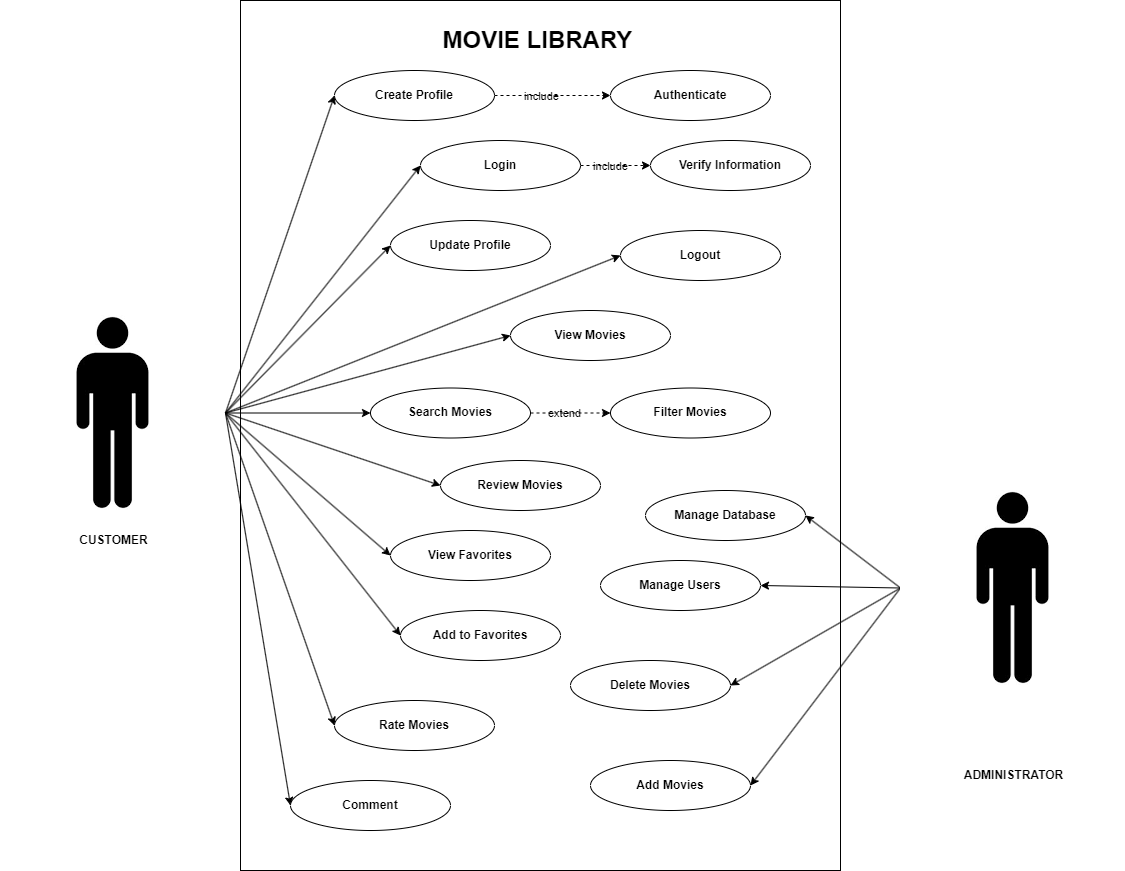
\includegraphics[scale=0.40]{images/USE CASE WET.drawio.png}\\[0.1cm] 

\clearpage
\myparagraph{Appendinx 2} ERD Classes

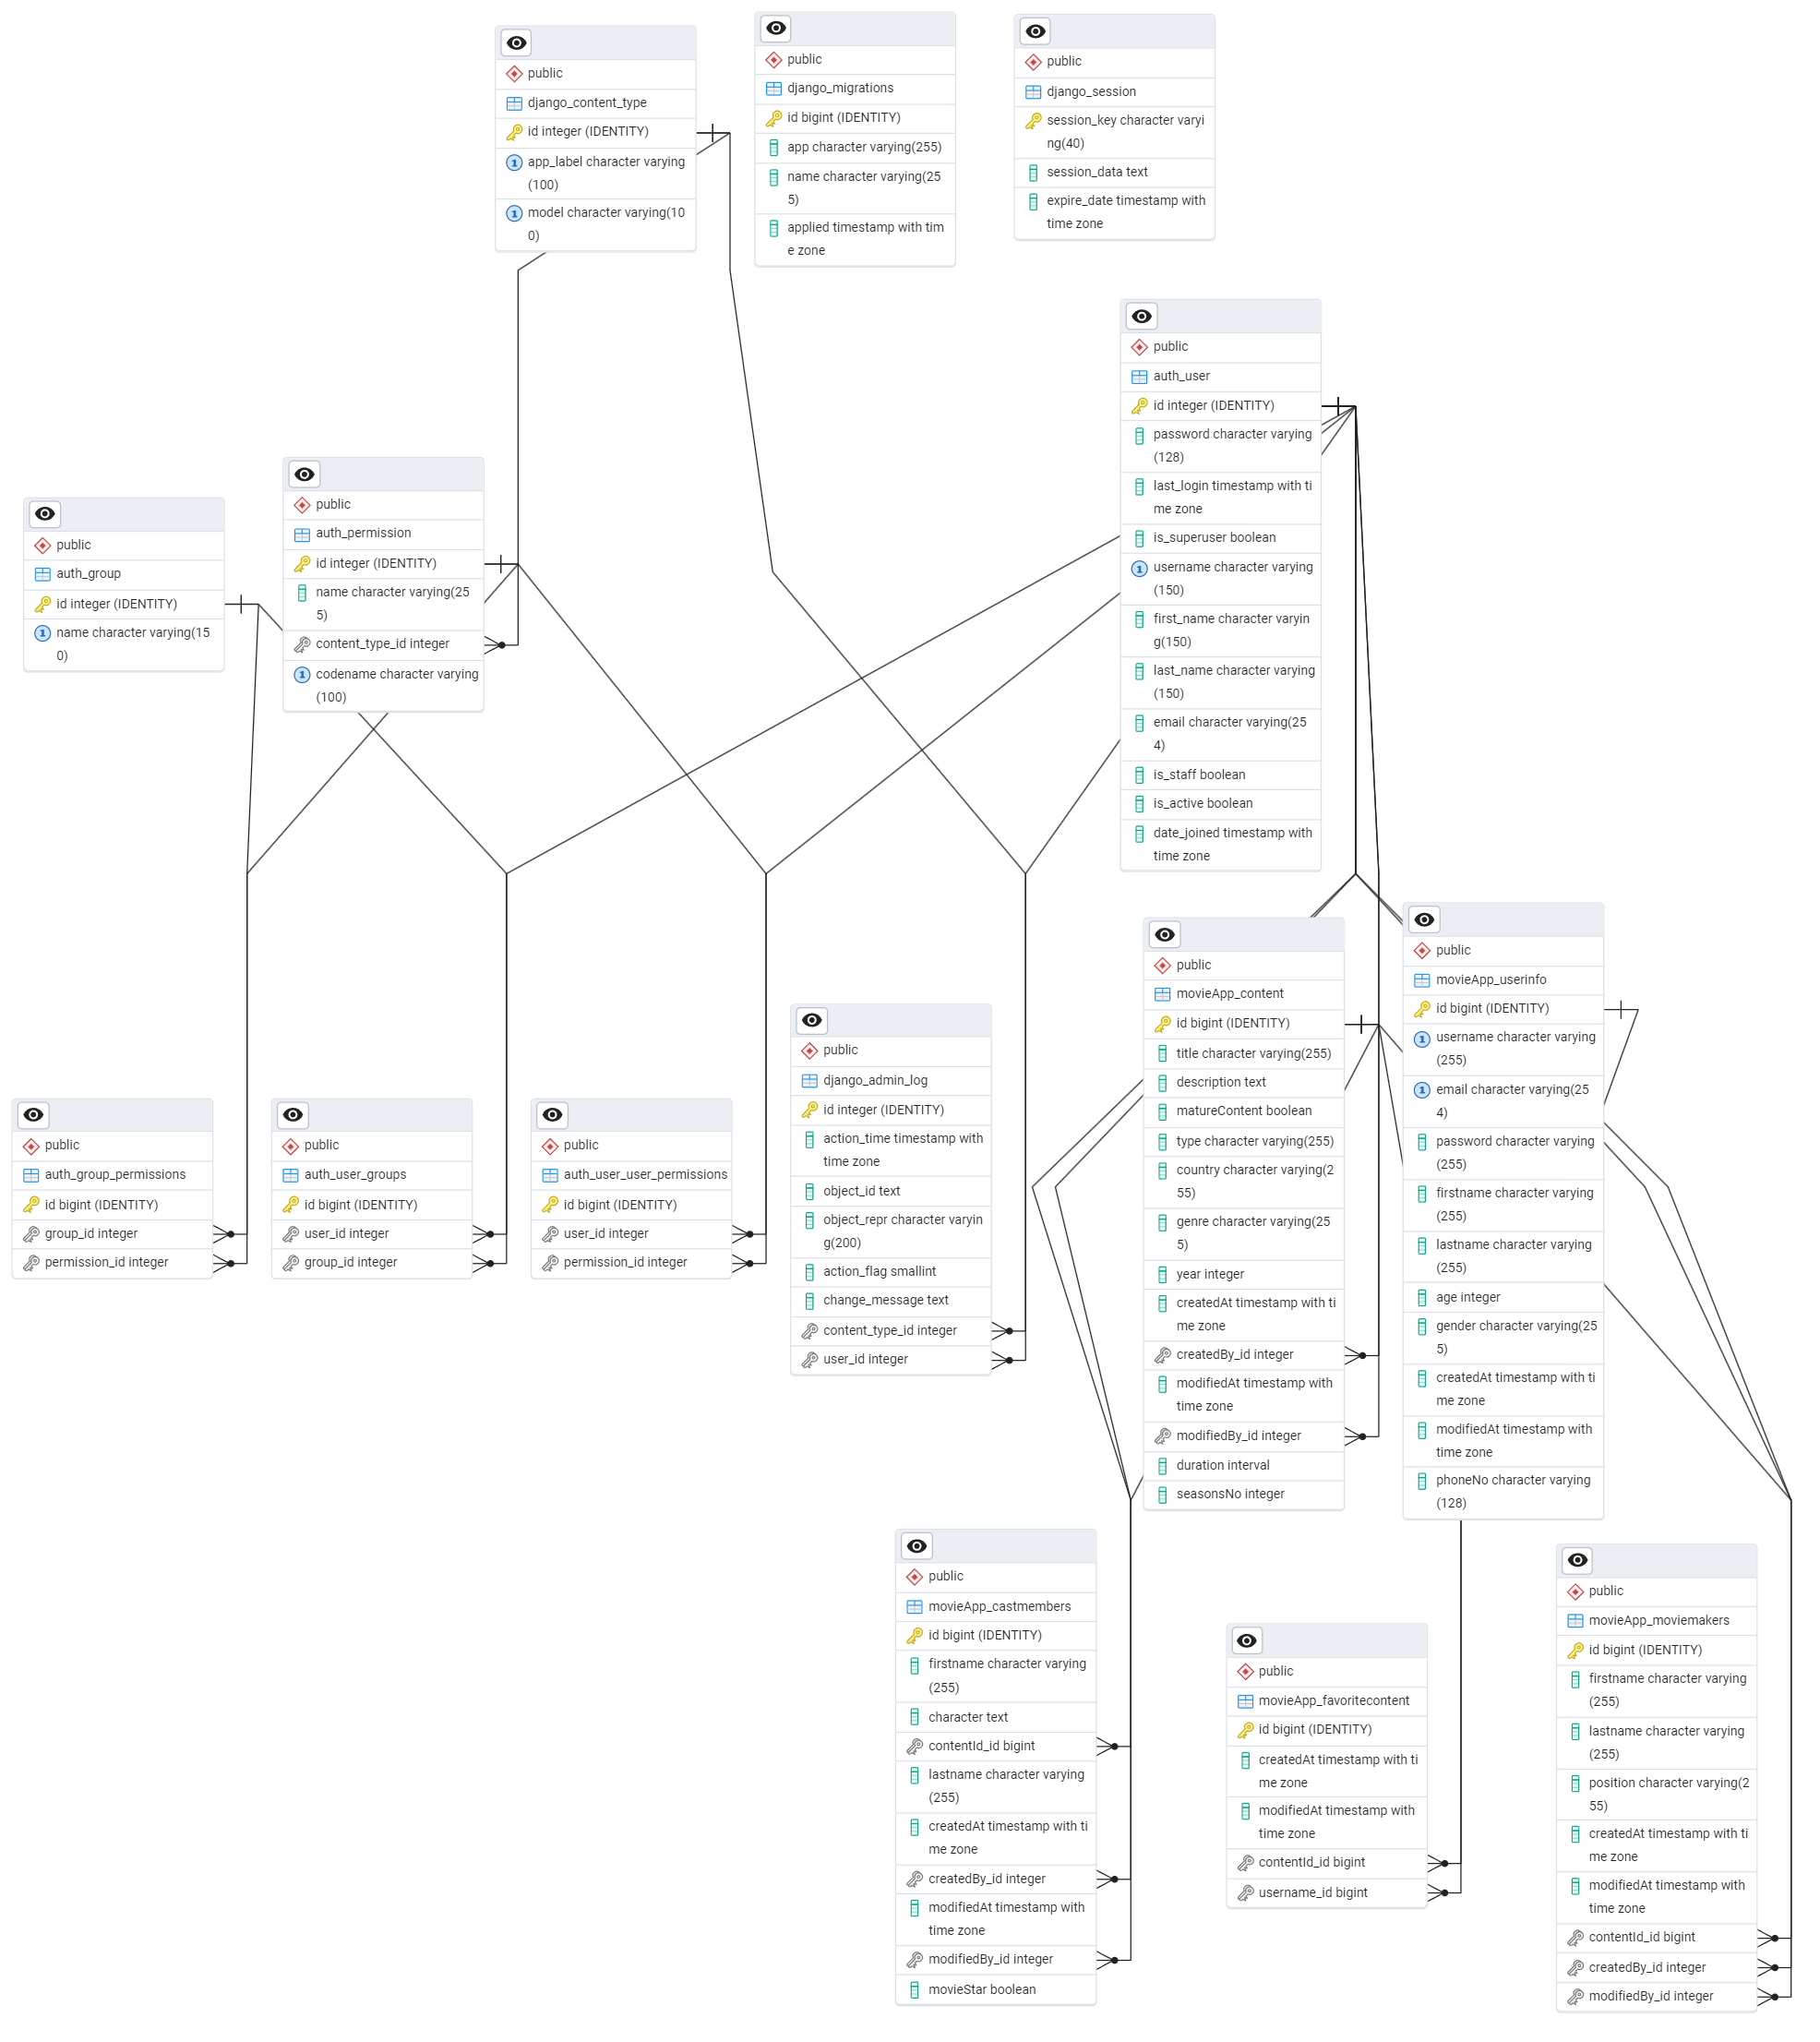
\includegraphics[scale=0.24]{images/ERDNewUpdated.png}\\[0.1cm] 

\clearpage
\myparagraph{Appendix 3} ERD Overview
\vspace{2ex}


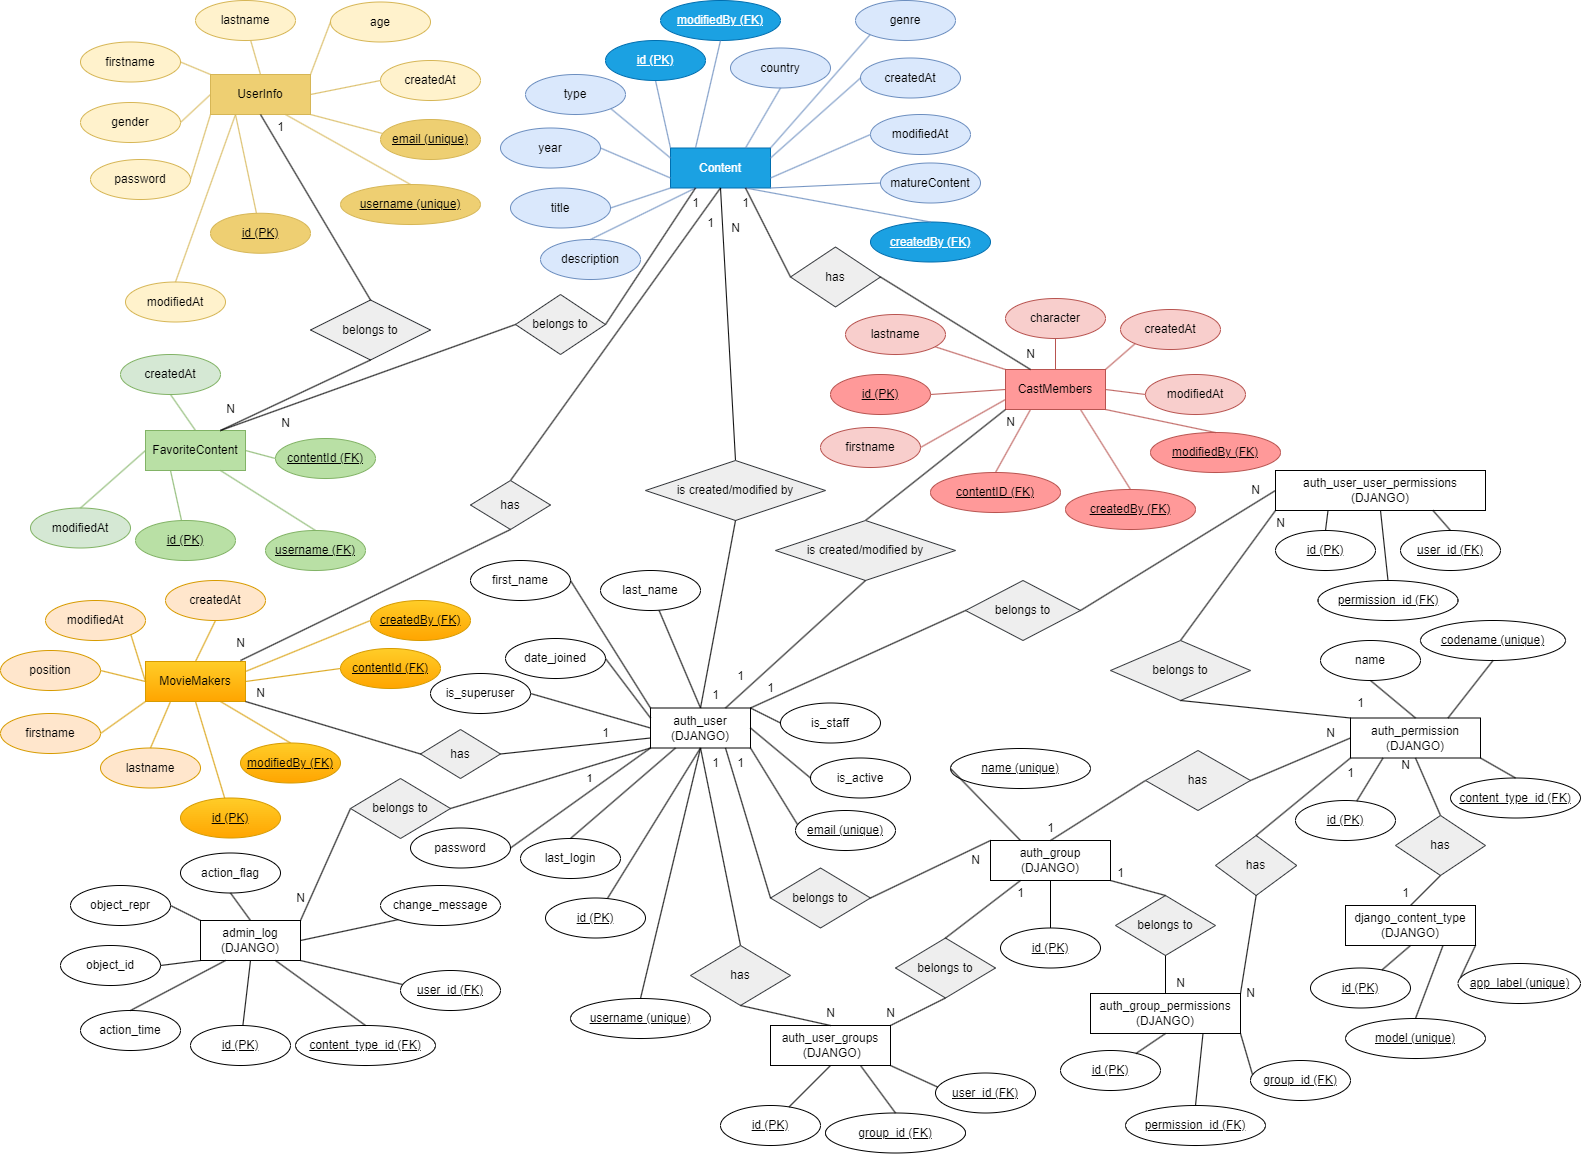
\includegraphics[scale=0.30]{images/WebTechERDNewUpdated.drawio.png}\\[0.1cm] 

\clearpage
\myparagraph{Appendix 4} API Viewset Example
\vspace{2ex}

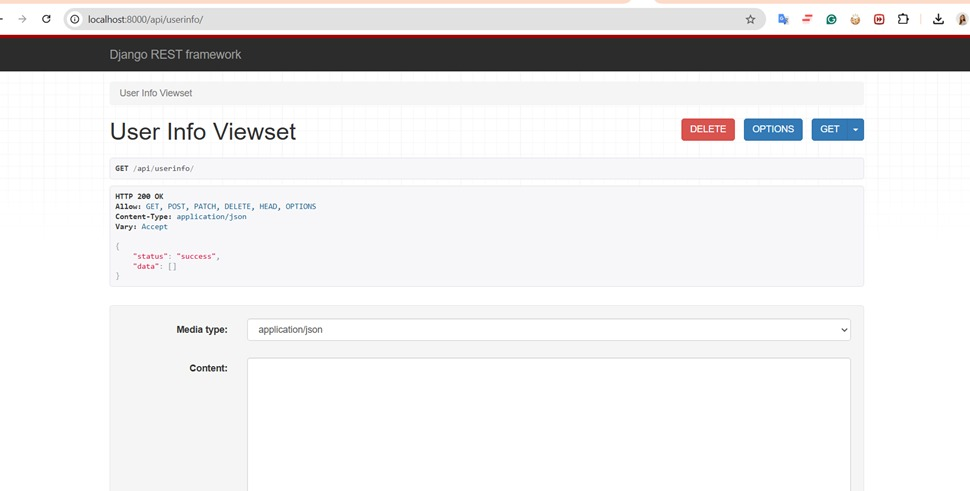
\includegraphics[scale=0.5]{images/WhatsApp Image 2024-12-13 at 16.01.10.jpeg}\\[0.1cm] 

\end{document}
